\documentclass{report}

\usepackage{graphicx}
\usepackage{hyperref}
\usepackage{tikz}
\usepackage{pgfplots}


\author{Mihalache Radu-Stefan}
\title{Study of functions using Hill Climbing and Simulated Annealing algorithms}

\begin{document}
\maketitle

\section{Introduction}
\subsection{Motivation}
The problem of exploring the values of functions and finding the global minimum of said function for a specified domain has useful aplications, yet it is dificult to solve with a deterministic algorithm.
That is because some functions have a very steep path to the minimum, like in the example below.

\begin{figure}[!h]
  \centering
\begin{tikzpicture}
  \begin{axis}[
      xlabel=x,
      ylabel=$f(x)$
    ]
    \addplot [
      color=red,
      mark=x
    ]
    coordinates {
      (0, 5)
      (1, 5.1)
      (2, 5.2)
      (3, 5.3)
      (3.3, 0)
      (3.5, 5.4)
      (7, 5.5)
    };
  \end{axis}
\end{tikzpicture}
\end{figure}

\section{Method}

Nondeterministic algorithms can be used to overcome this problem, as they have a better chance to explore the function and find the minimum . 
\newline
The representation of the input variables will be a string of n bits such that they can accuately represent the function domain.

$$x = a + decimal_{represenation}(bit_{str}) \cdot (b - a)/(2^n - 1) ,  x \in \left[a, b \right]$$

Using this represenattion, a random input called candidate solution can be generated, and its vecinity can be explored by negating one bit, such that the hamming distance between the candidate solution and the vecinity is one. This leads to the following aproaches:
\newline
\newline
Hill Climbing:
\newline
\newline
Select a candidate solution for each iteration and try to improove it using either the first better vecinity or the best vecinity. This algorithm finds the minimumm by exploring the basin of the candidate solution.
\newline
\newline
Simulated annealing:
\newline
\newline
Select a candidate solution at the start and explore its vecinity. This algorithm better explores the domain of the function by choosing worse vecinities base on the probability given by this expression:
\newline
$$random.uniform(0, 1) < math.exp(-abs((evaln - evalc) / temperature))$$
\newline
This algorithm makes use of the hot iron concept. At the begining the temperature  is high and the chance to choose a worse solution is high but it decreeses over each iteration based on this formula:
\newline
$$temperature = temperature * 0.9$$


\section{Experiment}

For this experiment, a python program will analyse theese functions on 5, 10 and 30 dimensions with $10^{-5}$ precissionn. Each test is run 30 times to ensure consistancy

\begin{figure}[!h]
  \centering
  $$ f(x) = \sum_{i=1}^n \left[ x_i^2 \right],
   x_i \in \left[ -5.12, 5.15 \right]$$

  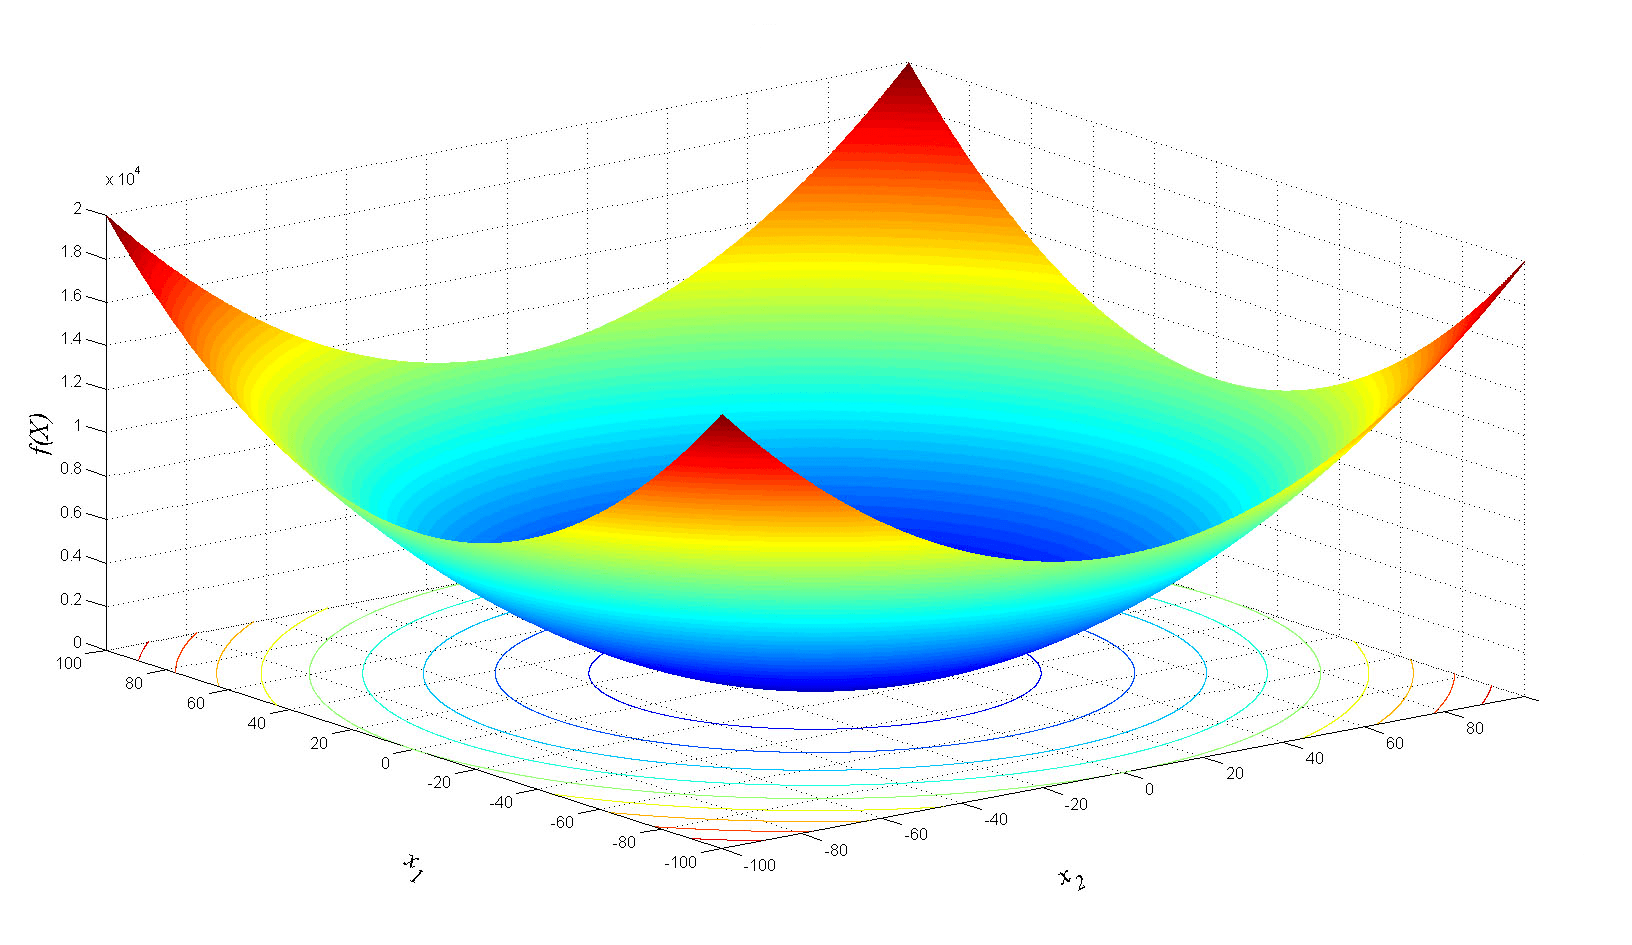
\includegraphics[width=100mm,scale=0.5]{De_Jong_function}
  \caption{Image De Jong's Function.\protect\footnotemark}
\end{figure}

\begin{figure}[!h]
  \centering
  $$ f(x) = \sum_{i=1}^n \left[-x_i \cdot sin(sqrt(|x_i|)) \right],
   x_i \in \left[ -500, 500 \right]$$

  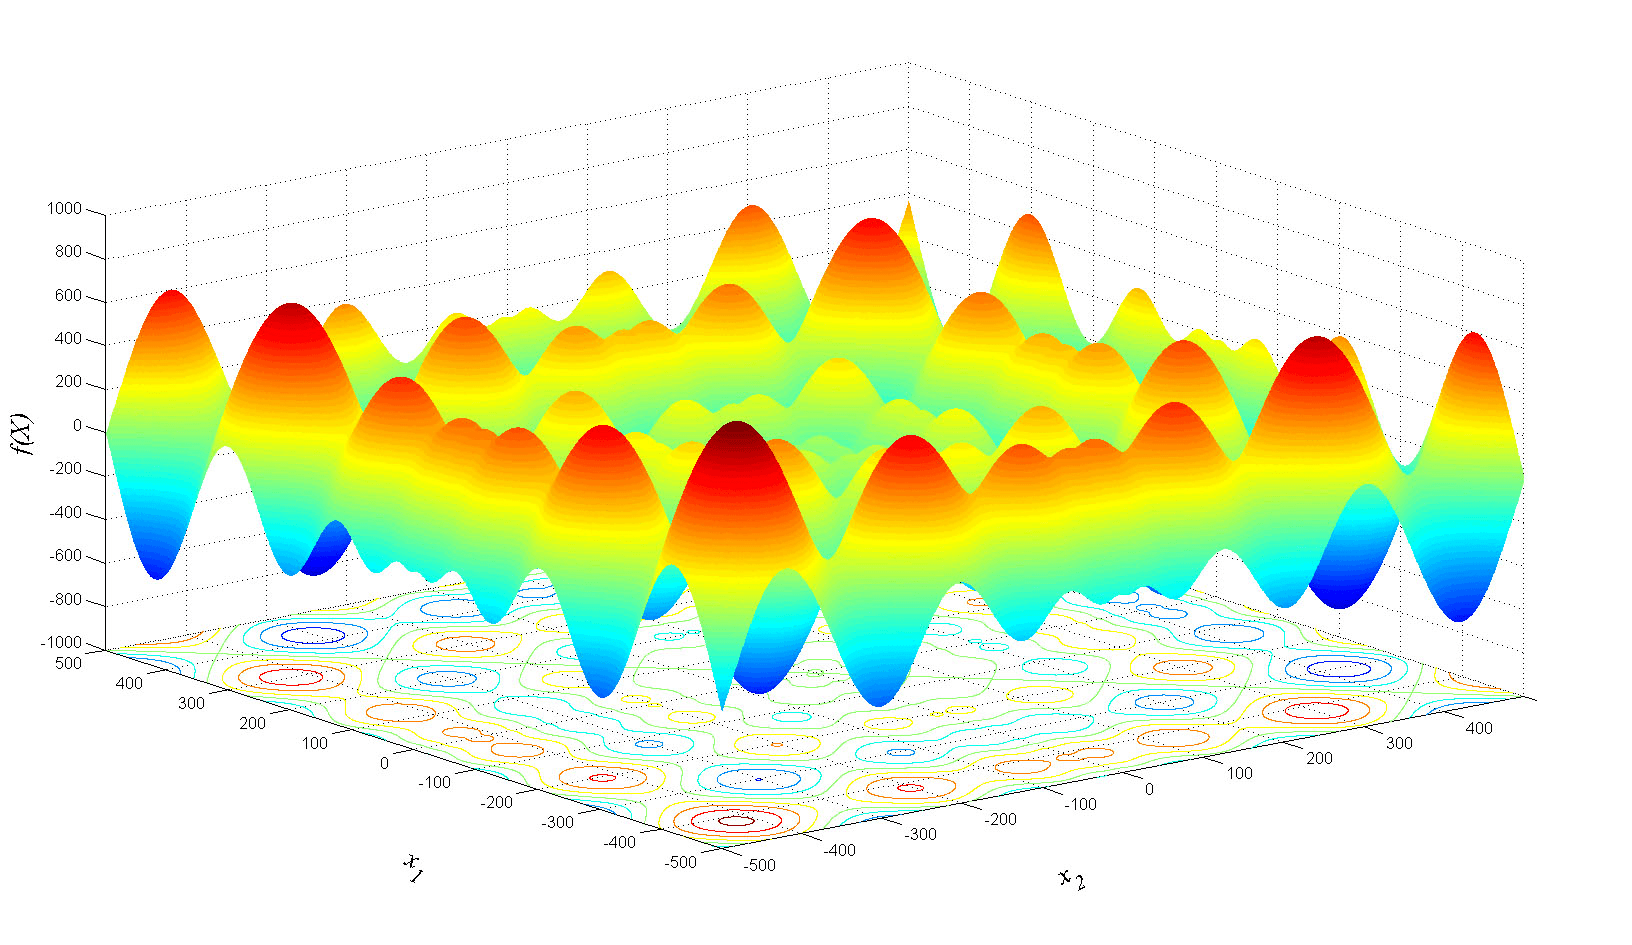
\includegraphics[width=100mm,scale=0.5]{Schwefel_fucntion}
  \caption{Image Schwefel's Function. \protect\footnotemark}
\end{figure}

\begin{figure}[!h]
  \centering
  $$ f(x) = A \cdot n + \sum_{i=1}^n \left[ x_i^2 - A \cdot cos(2 \pi x_i) \right],
  A = 10, x_i \in \left[ -5.12, 5.15 \right]$$

  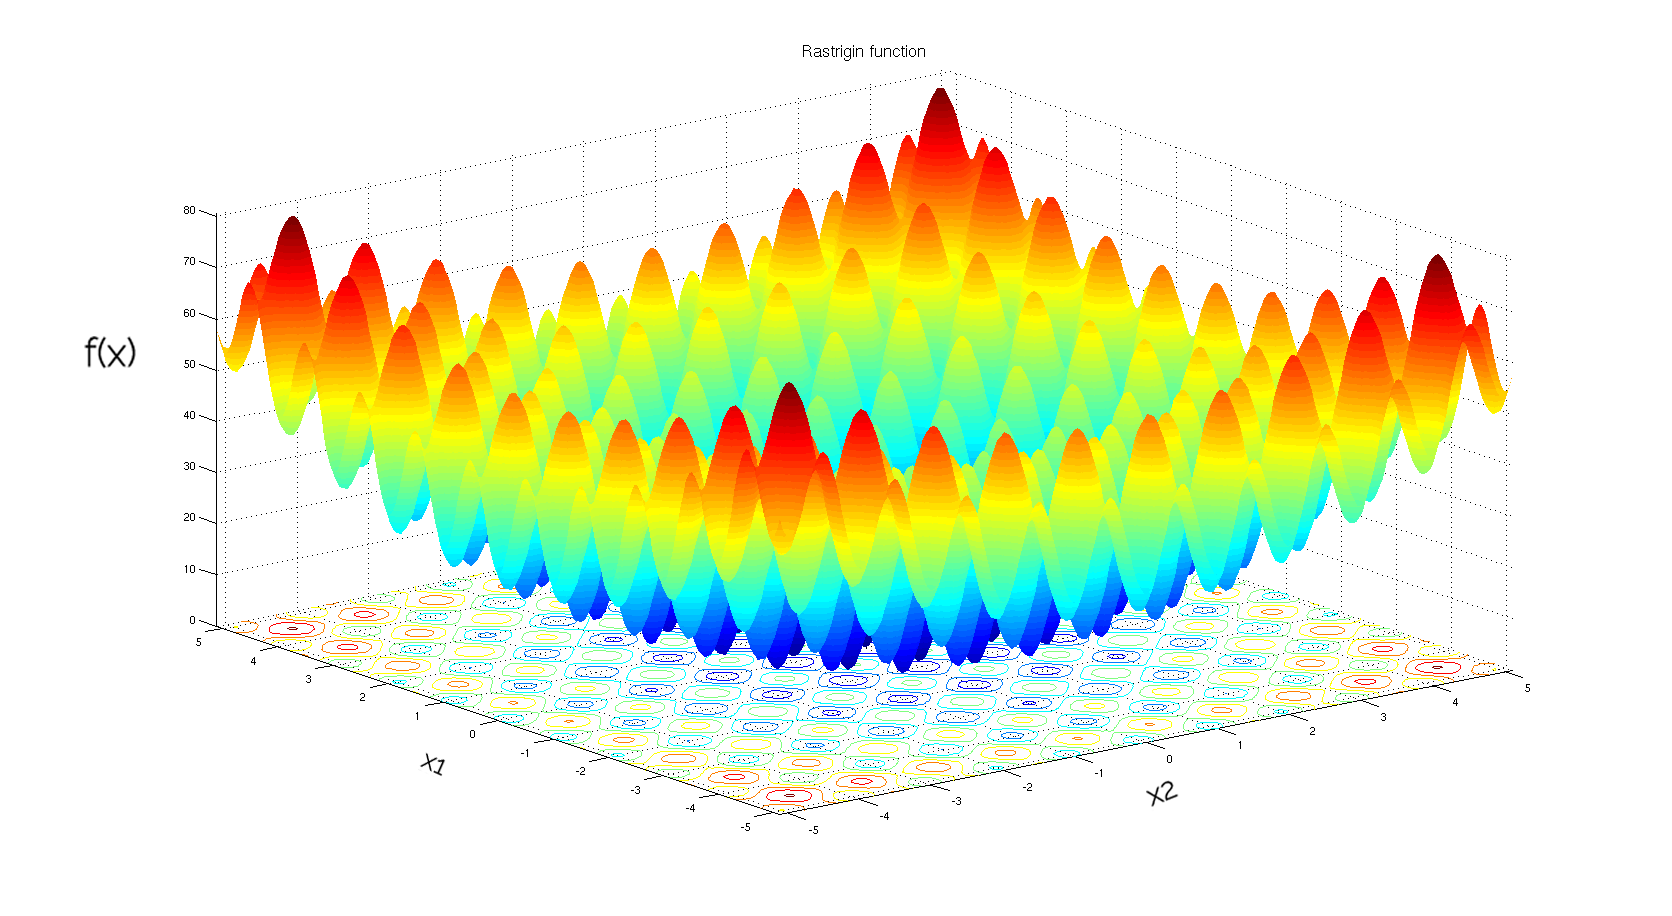
\includegraphics[width=100mm,scale=0.5]{Rastrigin_function}
  \caption{Image Rastrigin's Function. \protect\footnotemark}
\end{figure}

\begin{figure}[!h]
  \centering
  $$ f(x) = -\sum_{i=1}^n \left[sin(x_i) \cdot \left( sin\left( \frac{i \cdot x_i^2}{\pi}  \right) \right)^{2 \cdot m} \right] ,
  x_i \in \left[ 0, \pi \right] ,  m = 10$$

  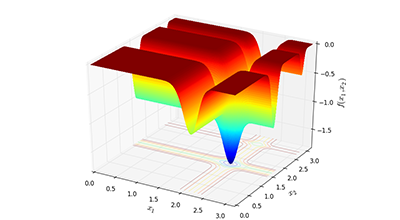
\includegraphics[width=100mm,scale=0.5]{Michalewicz_functions}
  \caption{Michalewicz's Function. \protect\footnotemark}
\end{figure}

\pagebreak

\section{Results}

\begin{figure}[!h]
\begin{tabular}{||c|||l|l||l||l||}
  \hline
  function & avg & min & max & time\\ \hline \hline
DeJong 1 5D - Hill Climbing first & 0 & 0 & 0 & 7 \\ \hline
DeJong 1 5D -Hill Climbing  best & 0 & 0 & 0 & 14 \\ \hline
DeJong 1 5D - Simulated Annealing  & 0 & 0 & 0 & 2 \\ \hline

DeJong 1 10D - Hill Climbing first & 0 & 0 & 0 & 56 \\ \hline
DeJong 1 10D - Hill Climbing best & 0 & 0 & 0 & 108 \\ \hline
DeJong 1 10D - Simulated Annealing & 0 & 0 & 0 & 4 \\ \hline

DeJong 1 30D - Hill Climbing first & 0 & 0 & 0 & 973 \\ \hline
DeJong 1 30D - Hill Climbing best & 0 & 0 & 0 & 1485 \\ \hline
DeJong 1 30D - Simulated Annealing & 0 & 0 & 0 & 10 \\ \hline

Schwefel 5D - Hill Climbing first & -1939 & -1992 & -1853 & 11 \\ \hline
Schwefel 5D -Hill Climbing  best & -1967 & -2094 & -1893 & 10 \\ \hline
Schwefel 5D - Simulated Annealing & -1825 & -1963 & -1776  & 3 \\ \hline

Schwefel 10D - Hill Climbing first & -3652 & -3872 & -3492 & 131 \\ \hline
Schwefel 10D -Hill Climbing  best & -3623 & -3772 & -3506 & 83 \\ \hline
Schwefel 10D - Simulated Annealing & -3642 & -3905 & -3246  & 7 \\ \hline

Schwefel 30D - Hill Climbing first & -9453 & -9923 & -9369 & 1525 \\ \hline
Schwefel 30D -Hill Climbing  best & -10153 & -10453 & -10063 & 1511 \\ \hline
Schwefel 30D - Simulated Annealing & -9746  & -11279 & -9365  & 20 \\ \hline

Rastrigin 5D - Hill Climbing first & 2.59497 & 1.88367 & 3.69702 & 13 \\ \hline
Rastrigin 5D -Hill Climbing  best & 2.23592 & 1.579144 & 2.98702 & 14 \\ \hline
Rastrigin 5D - Simulated Annealing & 2.23086 & 1.71005 & 3.102193 & 3 \\ \hline

Rastrigin 10D - Hill Climbing first & 7.18790 & 3.93217 & 15.19234 & 161 \\ \hline
Rastrigin 10D -Hill Climbing  best& 8.18790 & 3.67834 & 14.0925 & 121 \\ \hline
Rastrigin 10D - Simulated Annealing & 9.18790 & 3.19593 & 15.2394 & 7 \\ \hline

Rastrigin  30D - Hill Climbing first & 23.72184 & 17.12235 & 38.63187 & 1617 \\ \hline
Rastrigin  30D -Hill Climbing  best & 22.43780 & 16.97201 & 37.29053 & 1392 \\ \hline
Rastrigin  30D - Simulated Annealing & 25.18790 & 17.67834 & 38.44140 & 21 \\ \hline

Michalewicz 5D - Hill Climbing first & -4.44109 & -4.62793 & -3.97123 & 11 \\ \hline
Michalewicz 5D -Hill Climbing  best & -4.37306 &  -4.65685 & -4.02012 & 10 \\ \hline
Michalewicz 5D - Simulated Annealing & -4.28916 & -4.6328 & -3.26917 & 2 \\ \hline

Michalewicz 10D - Hill Climbing first & -8.20880 & -9.01029 & -6.89132 & 107 \\ \hline
Michalewicz 10D -Hill Climbing  best & -9.09037 &  -9.24031 & -8.25910 & 79 \\ \hline
Michalewicz 10D - Simulated Annealing & -8.70903 & -9.22690 &  -6.15737 & 6 \\ \hline

Michalewicz 30D - Hill Climbing first & -20.79776 & -22.61219 & -17.31592 & 560 \\ \hline
Michalewicz 30D -Hill Climbing  best & -24.09166 & -25.14376 & -22.21472 & 423 \\ \hline
Michalewicz 30D - Simulated Annealing & -23.66259 & -24.29173 & -21.53991 & 15 \\ \hline

  
\end{tabular}
\end{figure}



\subsection{Interpretation}

 Hill Climbing with the first and best neighbour choice give different resaults and times for different functions. Yet in all of them the time to solve large inputs is high in the python implementation that was used.
However, the simulated annealing approach gives marginally worse resaults and significanly better time. 

\section{Conclusions}
As demonstrated in the experiment, nondeterministic algorithms can be used to find the global minimum of functions.


\begin{thebibliography}{9}

\bibitem{wikipedia}
  Wikipedia Commons \\ Rastrigin's Function rendered image.
  \url{https://commons.wikimedia.org/wiki/Main_Page}

\bibitem{Al-roomi}
  Al-roomi  \\ De Jong's Function rendered image.
  \url{https://al-roomi.org/benchmarks/unconstrained/n-dimensions/}
  Al-roomi  \\ Schwefel's Function rendered image.
  \url{https://al-roomi.org/component/tags/tag/schwefel-function}

\bibitem{Sfui}
   Sfu \\ Michalewicz's Function rendered image.  
\url{https://www.sfu.ca/~ssurjano/michal.html}


\bibitem{Geatbx}
  Geatbxi  \\ Function formulas.
  \url{http://www.geatbx.com/docu/fcnindex-01.html}

\bibitem{Course}
  Course Page.
  \url{https://profs.info.uaic.ro/~eugennc/teaching/ga/l}

\bibitem{Pychard}
  Pychard.
  \url{https://www.jetbrains.com/pycharm/}


\end{thebibliography}  
\end{document}
